\newpage
\section{The Impact of Language and Improvisation}
\label{sec:data}
Training and validating models for research is usually done on the same dataset. This leads to solid proof-of-concept models, but can produce models that do not generalize well to real world scenarios. 

Another aspect of robustness of FER models against speech, which is the language dimension. We want to provide a platform to test our models against a different language, to see if this modality impacts performance. In this section we will present our approach to build a small database in German along the lines of RAVDESS. The datasets we used in this thesis are all recorded in English, and by comparing the performance of the models on the German recordings we can gain insights into their language dependency (Section \ref{sec:multilingual}). 

Another point to note is that the datasets we used are scripted and acted. Real world situations are not as rigid and more closely follow speech acts. We also collect videos of speech-acts that more closely resemble those of real world scenarios to later validate our models on them.

\subsection{Recording Setup}
We used the TAWNY recording tool \cite{tawny2021} for data collection. Each database was set up in a separate project. The participants recorded the videos themselves from home. Each recording was preceded with an information card (Figure \ref{fig:infocards}) which described the task for each video. The participants were given time to prepare their statements and could start their recording at their chosen time. Since the participants had to record themselves through a web browser application, the quality of videos varied depending on the available equipment.

\begin{figure}
    \centering
    \begin{subfigure}[b]{0.45\textwidth}
      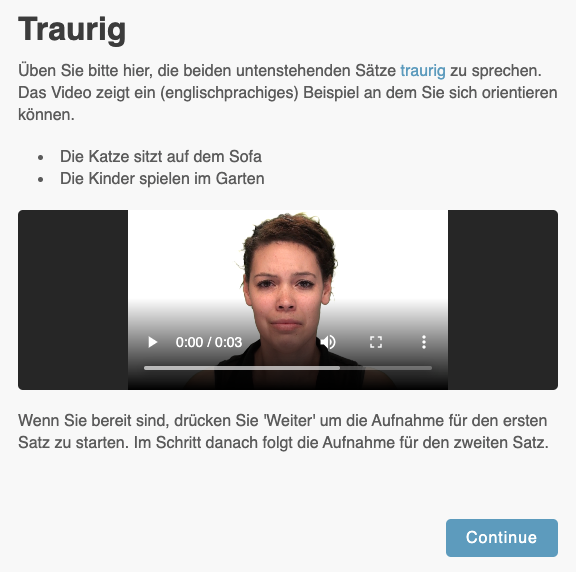
\includegraphics[width=\textwidth]{res/ger_ex.png}
    \end{subfigure}
    \begin{subfigure}[b]{0.45\textwidth}
      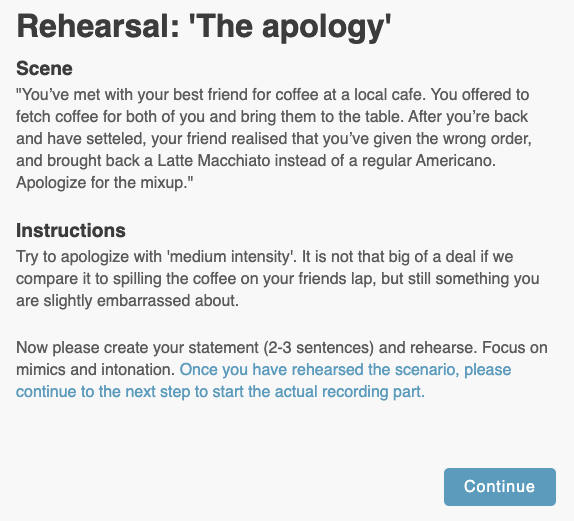
\includegraphics[width=\textwidth]{res/impro_ex.png}
    \end{subfigure}
    
    \caption{Information cards for each database project (Left: German RAVDESS, Right: Real World Speech Acts). The cards described the task for the following recording.}
    \label{fig:infocards}
\end{figure}

The videos were stored on the TAWNY platform \cite{tawny2021platform}, a SaaS emotion analytics platform, and were available for download after the participant concluded the recording of the given task.

\subsection{German RAVDESS - GRD}
\label{sec:german}

The lexical content of RAVDESS is kept simple. The actors speak two easy to pronounce sentences in eight emotions. We replicate this by switching the English sentences for German counterparts. We chose the two neutral statements "Die Katze sitzt auf dem Sofa" and "Die Kinder spielen im Garten", two sentences with eight syllables and commonly used words. The emotions are the same as in the RAVDESS database: neutral, calm, happy, sad, angry, fearful, surprise, and disgust.

Recordings were done using the TAWNY recording tool \cite{tawny2021}. The actors were given a general description of the task before starting their session. Before each individual recording the actors were given the target sentence and emotion, alongside an example from the RAVDESS dataset. The recordings were split, as the actors recited one statement per take. 

14 actors participated, 8 female and 6 male. We checked the videos for visual quality and sufficient emotional perception. After quality assessment, we end up with 141 recordings from 11 actors.

\subsection{Real World Speech Acts}
\label{sec:rwsa}
We want to figure out the impact of real world speech acts on our models and the emotional state of subjects. Compared to other datasets we use, the recordings in this collection do not have an underlying emotion. The emotional state should be induced by the statement and situation itself rather than from a scripted and ordered statement.

To collect statements that fit in real world scenarios, we put the actors in situations where they had to react with their own words. Four scenarios were built to produce certain responses:

\begin{enumerate}
    \item \textbf{Promise} "Together with one of your coworkers, you have just finished your lunch at a local restaurant. When it is time to pay, you realise that you forgot your wallet at the office. Knowing how stingy your colleague can be, try to ask him if you could borrow some money and affirm that you will give it back once you’re back at work."
    \item \textbf{Order} "You are the team lead of the sales team. You currently have the weekly meeting with your team members. Given that the yearly report is about to be due, it’s a very important week ahead. Remind Thomas that he is in charge of creating the final draft of the report, and tell him that it is due until next Friday."
    \item \textbf{Apology} "You’ve met with your best friend for coffee at a local cafe. You offered to fetch coffee for both of you and bring them to the table. After you’re back and have settled, your friend realised that you’ve given the wrong order, and brought back a Latte Macchiato instead of a regular Americano. Apologize for the mixup."
    \item \textbf{Assessment} "You are the team lead of the sales team. After a long and busy week, you meet with your team members for a debrief. Thomas has done a great job on the final draft of the yearly report, which he handed in on time. Compliment him on his great work."
\end{enumerate}

The recordings were collected with the TAWNY recording tool \cite{tawny2021}. The actors were confronted with the situation, and had time to make up a response before being recorded. Five people participated, one male and four female. After quality assessment, the recordings of only four participants were deemed usable. This is unfortunately not enough for detailled analysis.

\subsection{Discussion}
\label{sec:data_discussion}
\subsubsection{Multilingual Performance}
\label{sec:multilingual}
We validated our models on the videos of the GRD dataset from section \ref{sec:german}. The models for 90 frames could not be used since the videos were too short. The general trend from section \ref{sec:cross_dataset} is confirmed. The FER-TC model and the FER-SE model perform increasingly better with higher frame-window size. The FER-LN models performance does not increase with more temporal information. Compared to the results from section \ref{sec:cross_dataset} there is another decrease in accuracy, of around 10 percentage points. It is however not conclusive if this decrease is due to the language switch or other factors:
\begin{itemize}
    \item The recordings are not of the same quality as those of CREMA-D. For practical reasons all recordings had to be done remotely by the actors themselves using the TAWNY recording tool.
    \item The preparation of the actors were not comparable to those on CREMA-D. We did not have stimuli to actually put the actors into the desired emotional state and relied on their acting ability to convey the emotion.
    \item The actors only had one take to record their statements. Producers of other datasets generally have the capacity to have multiple takes for each recording.
\end{itemize}

\begin{figure}
    \centering
    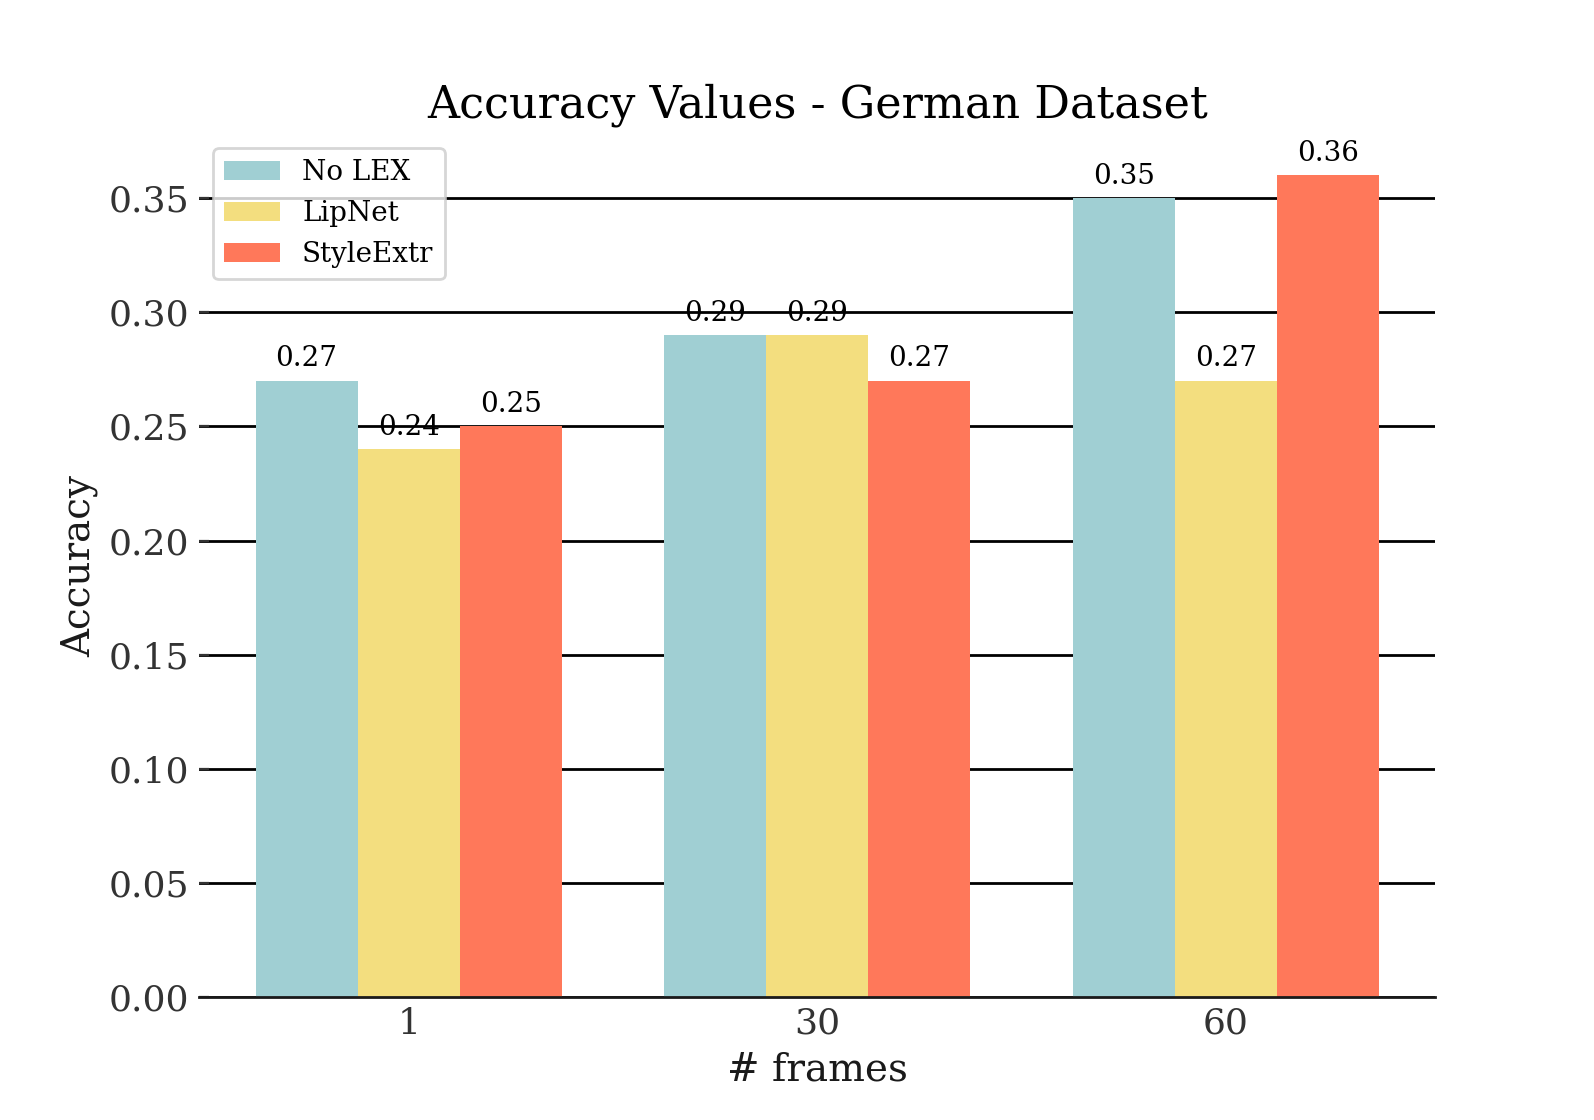
\includegraphics[width=0.8\textwidth]{res/GermanResults.png}
    \caption{Evaluating the models we trained on the GRD dataset from section \ref{sec:german}.}
    \label{fig:german_res}
\end{figure}

We can conclude that our models can adapt to recordings in German without much trouble. We would expect to see usable and comparable results with a dataset of another language given similar quality.

\subsubsection{Improvised Data}
The data collected in section \ref{sec:rwsa} was not extensive enough to provide any evaluation. Nevertheless we want to discuss the possibilities for analysis and our collection method.

We collected the data remotely with the TAWNY recording tool. The stimuli that described the scenarios (Section \ref{sec:rwsa}) were given in text form, and the actors had time to prepare their responses. Given that we want an improvised reaction that is not scripted, we suggest that the setup and introduction to the scenario should rather be given in a sketched video to immerse the actor into the situation. The response should also be given immediately without any time to prepare the statement.

To analyse the recordings, we would first need labels for the recordings. Since the statements were not induced by a predefined emotion, the labels would have to be manually added in postprocessing by human annotators. Since its possible that there are several emotional states during one recording, we would have the ability to detect and evaluate emotional shifts during speech, and analyse how our models cope with them. 